\documentclass[12pt]{article}
\usepackage{tikz}
\usepackage{xspace}
\usepackage{wrapfig}
\usepackage{stackengine}
\usepackage{roundrule}
\usepackage{bm} % for bold math symbols
\usepackage{multicol} % for multiple columns
\usepackage{hyperref} % for links

\textwidth      165mm
\textheight     242mm
\topmargin      -18mm
\oddsidemargin  -2mm
\evensidemargin -2mm
\pagestyle{empty}
\renewcommand{\baselinestretch}{0.96}
\renewcommand{\theenumi}{\alph{enumi}}

\newcommand{\false}{\ensuremath{\mathbf{f}}\xspace}
\newcommand{\true}{\ensuremath{\mathbf{t}}\xspace}
\newcommand{\impl}{\mathbin{\Rightarrow}}
\newcommand{\biim}{\mathbin{\Leftrightarrow}}

% Defining digits in display style (credit to S. B. Segletes)

\setstackEOL{\\}
\setstackgap{S}{0pt}
\def\barThk{0.75pt}% rule thickness
\def\barLen{3.75pt}% rule length
\def\barGap{.3pt}% rule gap
\def\barsb{0.75pt}% character sidebearing
\newcommand\barlet[2]{\def#1{\kern\barsb\Shortstack{#2}\kern\barsb}}

\def\barX{\smash{%
  \kern\barGap\roundrule[-.5\dimexpr\barThk]{\barLen}{\barThk}\kern\barGap}}
\def\barY{\makebox[0pt]{\raisebox{\barGap}{%
  \addstackgap[\barGap]{\roundrule{\barThk}{\barLen}}}}}
\def\barXP{\kern\dimexpr\barLen+2\dimexpr\barGap\relax\relax}
\def\barYP{\rule{0pt}{\dimexpr\barLen+2\dimexpr\barGap\relax\relax}}

\barlet\barZero{\barX\\\barY\barXP\barY\\\barY\barX\barY}
\barlet\barOne{\barXP\\\barXP\barY\\\barXP\barY}
\barlet\barTwo{\barX\\\barX\barY\\\barY\barX}
\barlet\barThree{\barX\\\barX\barY\\\barX\barY}
\barlet\barFour{\barXP\\\barY\barX\barY\\\barXP\barY}
\barlet\barFive{\barX\\\barY\barX\\\barX\barY}
\barlet\barSix{\barX\\\barY\barX\\\barY\barX\barY}
\barlet\barSeven{\barX\\\barXP\barY\\\barXP\barY}
\barlet\barEight{\barX\\\barY\barX\barY\\\barY\barX\barY}
\barlet\barNine{\barX\\\barY\barX\barY\\\barX\barY}
\barlet\barDash{\barXP\\\barX\\\barYP}

\begin{document}

\begin{center}
{\sc The University of Melbourne
\\
School of Computing and Information Systems
\\ 
COMP30026 Models of Computation}
\bigskip \\
{\Large\bf Assignment 1, 2019}
\bigskip \\
{\large Released: 27 August.  Deadline: 15 September at 23:00}
\end{center}

\section*{Purpose}
To improve your understanding of propositional logic, first-order 
predicate logic, mechanized reasoning, and discrete mathematics.
To develop skills in analysis and formal reasoning about complex concepts,
and to practise writing down formal arguments with clarity.

% \section*{Six challenges}

\subsection*{Challenge 1}
Consider the four first-order predicate formulas
\[
\begin{array}{lll}
   F & = & \forall x\ (\neg P(x,x))
\\ G & = &
    \forall x\ \forall y\ \forall z\ (P(x,y) \land P(y,z) \impl P(x,z))
\\ G' & = &
    \forall x\ \forall y\ \forall z\ (P(x,y) \land P(y,z) \impl \neg P(x,z))
\\ H & = & \forall x\ \forall y\ (P(x,y) \impl \neg P(y,x))
\end{array}
\]
\begin{enumerate}
\setlength{\itemsep}{-0.3ex}
\item
Show that $F \lor G \lor G' \lor H$ is not valid.
\item
Show that $F \land G' \land H$ is satisfiable.
\item
Show that $(F \land G) \impl H$ is valid.
\end{enumerate}

\subsection*{Challenge 2}

For this challenge use the following predicates:
\begin{itemize}
\setlength{\itemsep}{-0.5ex}
\item
$F(x)$, which stands for ``the force is with $x$''
\item
$J(x)$, which stands for ``$x$ is a Jedi master''
\item
$E(x,y)$, which stands for ``$x$ exceeds $y$''
\item
$P(x,y)$, which stands for ``$x$ is a pupil of $y$''
\item
$V(x)$, which stands for ``$x$ is venerated''
\end{itemize}
and use the constant `$a$' to denote Yoda.
\begin{enumerate}
\item
For each of the statements $S_1,\ldots S_4$, express it
\emph{as a formula in first-order predicate logic}
(not clausal form):
\begin{description}
\setlength{\itemsep}{-0.2ex}
\item[$S_1$:] ``The force is with every Jedi master.''
\item[$S_2$:] ``Yoda exceeds some Jedi master.''
\item[$S_3$:] ``A Jedi master is venerated if (1) the force is with 
              him/her \emph{and} (2) all his/her pupils exceed him/her.''
\item[$S_4$:] ``Every Jedi master without pupils as venerated.''
\end{description}
(Be careful to get these translations right, including $S_3$;
most of the following depends on this.)
\item
Translate $S_1$--$S_3$ to clausal form.
\item
Translate \emph{the negation of} $S_4$ to clausal form.
\item
Give a proof by resolution to show that $S_4$ follows from
the other statements.
\end{enumerate}

\subsection*{Challenge 3}

Let ${\cal B} = \{0,1\}$ be the set of Boolean values,
so that ${\cal B}^n$ is the set of $n$-tuples of Boolean values
(or Boolean \emph{vectors}).
We use a bold variable $\bm{b}$ to denote a Boolean vector
of $n$ Boolean values $(b_1, b_2, \ldots, b_n)$

An $n$-dimensional Boolean \emph{vector function}
$\bm{f} : {\cal B}^n \rightarrow {\cal B}^n$
is \emph{reversible} iff
for every Boolean vector $\bm{y} \in {\cal B}^n$
there is exactly one vector $\bm{x} \in {\cal B}^n$
such that $\bm{f}(\bm{x}) = \bm{y}$.
Intuitively, the function is reversible iff we can uniquely
determine the input vector from an output vector, allowing us
to reliably `reverse' the evaluation of the function.
For example, $\bm{f}(b_1, b_2) = (b_2, b_1)$ is a
2-dimensional reversible Boolean vector function, and
$\bm{g}(b_1, b_2) = (b_1 \land b_2, b_1 \lor b_2)$ is a
2-dimensional Boolean vector function that is not reversible
(because, for example, $(0, 1) = \bm{g}(0, 1) = \bm{g}(1, 0)$).

(This kind of logic function finds important applications in
the theory of quantum computation, where the laws of quantum
mechanics constrain computations to proceed reversibly.)

\begin{enumerate}
\item
Consider the Boolean vector function
$\bm{f_a}(b_1, b_2) = (\neg b_1, b_1 \oplus b_2)$.
Show that this function is reversible.

\item
Consider the Boolean vector function
$\bm{f_b}(b_1, b_2, b_3)
  = (b_1 \oplus b_2, b_2 \oplus b_3, b_3 \oplus b_1)$.
Show that this function is \emph{not} reversible.

\item
Is the Boolean vector function 
$\bm{f_c}(b_1, b_2, b_3)
  = (b_1 \oplus b_3, \neg b_3, b_1 \oplus b_2)$
reversible?
Justify your answer.

\item
Give a formula, in terms of $n$, for the fraction of distinct
$n$-dimensional Boolean vector functions that are reversible.

Note that two $n$-dimensional Boolean vector functions are
considered distinct iff they produce different output vectors
for some input vector. For example, we should not count
$\bm{f}(b_1) = (\neg b_1)$ and
$\bm{g}(b_1) = (b_1 \oplus \mathbf{t})$
as two distinct functions---despite syntactic differences,
$\bm{f}$ and $\bm{g}$ produce matching outputs for all inputs.
Here we are only interested in counting functions with
differing behaviour.
\end{enumerate}

\subsection*{Challenge 4}

Find ways to avoid unnecessarily complex propositional formulas:
\begin{enumerate}
\setlength{\itemsep}{-0.5ex}
\item 
Give the shortest possible formula that is equivalent to
$(P \impl Q) \impl \neg Q$.
\item 
Express $P \impl ((P \land Q) \impl R)$
using no connectives other than $\impl$.
\item 
Express $(P \impl (Q \lor R)) \land (P \biim Q)$
using no connectives other than $\biim$.
\end{enumerate}
The answers to this challenge must be submitted through Grok.
For each question, you are to submit the answer as a Haskell
expression of type \verb!Exp!, where \verb!Exp! is the type
of structure trees used for propositional formulas
in the second half of Worksheet 1 (see Grok).
For variable names (of type Char), use \verb!'P'!, \verb!'Q'!, and 
\verb!'R'!, that is, use upper case.

\subsection*{Challenge 5}

Consider the following light switching game. We begin with an $n$
by $n$ grid of square buttons, numbered 1--$n^2$, initially dark,
as shown below (left) for $n=4$.
Pressing any button will cause that button to light up, along with its
immediate neighbours above, below, and to its left and right in the
grid.
For example, the result of pressing button 11 is depicted below (middle).
Subsequent button presses will continue to light up nearby buttons, or
switch them back off if they are already alight.
For example, the result of pressing button 15 (after button 11) is shown
below (right).
Note that because buttons 15 and 11 were both alight, they became dark
again.
Note also that the grid does not `wrap around': button 15 has no effect
on button 3.
The aim of the puzzle, given a particular light configuration, is to
find a sequence of button-presses that will produce this configuration.
To help you familiarise yourself with this puzzle, we provide a grid
for the $n=4$ case at \url{https://comp30026.far.in.net/puzzle}.
\begin{center}
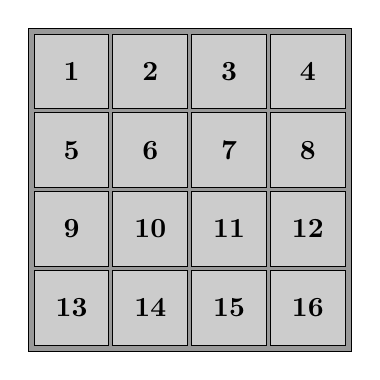
\begin{tikzpicture}
\draw[fill=black!40!white] (-0.55, -0.55) rectangle (3.55, 3.55);
\foreach \x/\y/\n in {0/3/1, 1/3/2, 2/3/3, 3/3/4,
                      0/2/5, 1/2/6, 2/2/7, 3/2/8,
                      0/1/9, 1/1/10,2/1/11,3/1/12,
                      0/0/13,1/0/14,2/0/15,3/0/16}
    \node[draw,minimum size=27,fill=black!20!white] 
	at (\x, \y) {\bf \n};
\end{tikzpicture}
\qquad\qquad
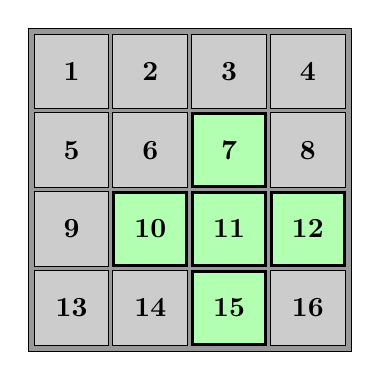
\begin{tikzpicture}
\draw[fill=black!40!white] (-0.55, -0.55) rectangle (3.55, 3.55);
\foreach \x/\y/\n in {0/3/1, 1/3/2, 2/3/3, 3/3/4,
                      0/2/5, 1/2/6, 2/2/7, 3/2/8,
                      0/1/9, 1/1/10,2/1/11,3/1/12,
                      0/0/13,1/0/14,2/0/15,3/0/16}
    \node[draw,minimum size=27,fill=black!20!white] (p\n) 
	at (\x, \y) {\bf \n};
\foreach \n in {7, 10, 11, 12, 15}
    \node[draw,minimum size=26,fill=green!30!white,thick]
        at (p\n) {\bf \n};
\end{tikzpicture}
\qquad\qquad
\begin{tikzpicture}
\draw[fill=black!40!white] (-0.55, -0.55) rectangle (3.55, 3.55);
\foreach \x/\y/\n in {0/3/1, 1/3/2, 2/3/3, 3/3/4,
                      0/2/5, 1/2/6, 2/2/7, 3/2/8,
                      0/1/9, 1/1/10,2/1/11,3/1/12,
                      0/0/13,1/0/14,2/0/15,3/0/16}
    \node[draw,minimum size=27,fill=black!20!white] 
	at (\x, \y) {\bf \n};
\foreach \n in {7, 10, 12, 14, 16}
    \node[draw,minimum size=26,fill=green!30!white,thick]
        at (p\n) {\bf \n};
\end{tikzpicture}
\end{center}
Your task is to write a Haskell program capable of solving this puzzle.
Given a grid size $n$ and a light configuration as input, your program
must output a sequence of buttons which, when pressed in order, will
produce the desired configuration.

The answer to this challenge must be submitted through Grok,
in the form of a function {\tt lights} of type {\tt Int -> [Int] -> [Int]}
The first input parameter provides the dimensionality of the puzzle grid,
$n$, and will always be a positive integer.
The second input parameter represents the buttons to be switched on in the
desired configuration (any buttons not listed are to be switched off).
The return value should be a list representing the sequence of buttons
to press in your solution to the puzzle, or, in case the configuration is
impossible to achieve, the return value should be an empty list.
For example, the input/output pair below corresponds to a 4 by 4 puzzle
in which the desired configuration is the one above (right), and to one
possible solution to this puzzle:
\begin{verbatim}
    > lights 4 [7, 10, 12, 14, 16]
    [11, 15]
\end{verbatim}

\emph{Hint 1}: Our suggested approach is for you to model the puzzle as
a propositional satisfiability problem. In this way, the task becomes a
simple translation from a puzzle description to a propositional formula,
and you can use tools like those you have constructed in assessed worksheets
1 and 2 to solve the formula itself (we provide similar tools on Grok).
The code required for this approach is minor compared to the code required
to implement a puzzle-specific search algorithm.

\emph{Hint 2}: There are many ways to approach this modelling task. 
To get you started on the right track, consider the following questions 
(assume $n=4$):
(1) What light configuration results from the sequence {\tt [15, 11]}?
How does this compare to the above example?
(2) What light configuration results from the sequence {\tt [6, 1, 6]}?
How about {\tt [6, 1, 6, 6]}? Is it ever useful to press a button more
than once?
(3) Could you determine the final state of a single button by looking at a
long sequence of button presses, without simulating the whole sequence?

\subsection*{Challenge 6}

Consider a single-digit display which will be used to show any
decimal digit, or a dash:
\begin{center}
\barZero,
\barOne,
\barTwo,
\barThree,
\barFour,
\barFive,
\barSix,
\barSeven,
\barEight,
\barNine,
\barDash 
\end{center}
Arrays of such displays are used to display numbers in 
digital clocks, washing machines and other devices.
A \emph{seven-segment} display is made up by seven LEDs 
(labelled $a$--$g$), as shown below on the right.
For example, to show the digit 3, all display segments except
$b$ and $e$ are lit up.

Each of the seven display segments a--g can be considered a propositional
function of four propositional variables $W$, $X$, $Y$ and $Z$, with
input $WXYZ$ specifying the desired decimal digit in binary notation
(or 1010 for a dash).
For example, input 3 is given by $WXYZ = 0011$ 
(that is, $W$ and $X$ are false and $Y$ and $Z$ are true).
For that input combination, the outputs $b$ and $e$ should be 0
(False) while the rest should be 1 (True).
Given this, the truth tables for all the functions $a$--$g$ are as 
shown in the table below.
\bigskip

\begin{minipage}{0.6\textwidth}
\qquad
$\begin{array}{|cccc|ccccccc|}
   W & X & Y & Z & ~a~ & ~b~ & ~c~ & ~d~ & ~e~ & ~f~ & ~g~
\\ \hline
   0 & 0 & 0 & 0 & 1 & 1 & 1 & 0 & 1 & 1 & 1 
\\ 0 & 0 & 0 & 1 & 0 & 0 & 1 & 0 & 0 & 1 & 0 
\\ 0 & 0 & 1 & 0 & 1 & 0 & 1 & 1 & 1 & 0 & 1 
\\ 0 & 0 & 1 & 1 & 1 & 0 & 1 & 1 & 0 & 1 & 1 
\\ 0 & 1 & 0 & 0 & 0 & 1 & 1 & 1 & 0 & 1 & 0 
\\ 0 & 1 & 0 & 1 & 1 & 1 & 0 & 1 & 0 & 1 & 1 
\\ 0 & 1 & 1 & 0 & 1 & 1 & 0 & 1 & 1 & 1 & 1 
\\ 0 & 1 & 1 & 1 & 1 & 0 & 1 & 0 & 0 & 1 & 0 
\\ 1 & 0 & 0 & 0 & 1 & 1 & 1 & 1 & 1 & 1 & 1 
\\ 1 & 0 & 0 & 1 & 1 & 1 & 1 & 1 & 0 & 1 & 1 
\\ 1 & 0 & 1 & 0 & 0 & 0 & 0 & 1 & 0 & 0 & 0 
\\ 1 & 0 & 1 & 1 & * & * & * & * & * & * & * 
\\ 1 & 1 & 0 & 0 & * & * & * & * & * & * & * 
\\ 1 & 1 & 0 & 1 & * & * & * & * & * & * & * 
\\ 1 & 1 & 1 & 0 & * & * & * & * & * & * & * 
\\ 1 & 1 & 1 & 1 & * & * & * & * & * & * & * 
\\ \hline
\multicolumn{10}{c}{~}
\end{array}$
\end{minipage}
\qquad
\begin{minipage}{0.3\textwidth}
\begin{center}
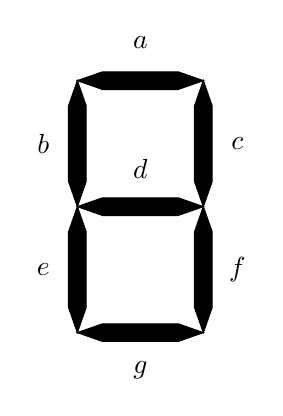
\begin{tikzpicture}
\begin{scope}[scale=0.16]

\path[draw,fill]%
(-5,1)--(-3,1.7)--(3,1.7)--(5,1)--(3,0.3)--(-3,0.3)--cycle;
\path[draw,fill]%
(-5,11)--(-3,11.7)--(3,11.7)--(5,11)--(3,10.3)--(-3,10.3)--cycle;
\path[draw,fill]%
(-5,21)--(-3,21.7)--(3,21.7)--(5,21)--(3,20.3)--(-3,20.3)--cycle;
\path[draw,fill]%
(5,1)--(4.3,3)--(4.3,9)--(5,11)--(5.7,9)--(5.7,3)--cycle;
\path[draw,fill]%
(5,11)--(4.3,13)--(4.3,19)--(5,21)--(5.7,19)--(5.7,13)--cycle;
\path[draw,fill]%
(-5,11)--(-4.3,13)--(-4.3,19)--(-5,21)--(-5.7,19)--(-5.7,13)--cycle;
\path[draw,fill]%
(-5,1)--(-4.3,3)--(-4.3,9)--(-5,11)--(-5.7,9)--(-5.7,3)--cycle;

\node at (-7.7,16) {$b$};
\node at (-7.7,6)  {$e$};
\node at (0,24)    {$a$};
\node at (0,14)    {$d$};
\node at (0,-2)    {$g$};
\node at (7.7,16)  {$c$};
\node at (7.7,6)   {$f$};

\end{scope}
\end{tikzpicture}
\end{center}
\end{minipage}

\noindent
An asterisk (*) in the table marks an output that we don't care about.
It is assumed that the last five input combinations will never 
happen, so we are free to let the corresponding outputs be 
whatever is convenient.

The single-digit display must be implemented with logic circuitry.
Here we assume that only three types of logic gates are available.
An \emph{and-gate} takes two inputs and produces, as output, the
conjunction ($\land$) of the inputs.
Similarly, an \emph{or-gate} implements disjunction ($\lor$).
Finally, an \emph{inverter} takes a single input and negates it.

The task here is to design a circuit for all of $a$--$g$ using as
few gates as possible.
We can specify the circuit by writing down the Boolean equations
for each of the outputs $a$--$g$.
For example, we can define 
$f = \neg (X \land \neg Y \land Z)$,
which shows that we can implement $f$ with as little as four gates.
Since we want to use as few gates as possible, it is important to
look for cases where outputs can be \emph{shared}, or reused.
For example, if we have already implemented $b$ then we could define
$f = b \lor Z$, using just one gate.
Note that for any sub-circuit that you want to share 
(that is, you want to direct its output to different places), 
the output must have a name.
You can define as many ``helper'' functions as you please, to
create the smallest possible solution.
For example, suppose you have implemented some function using
$\neg (X \lor Y)$ as a sub-circuit, and now you realise that
there is another function that could also use that sub-circuit.
Rather than duplicate the sub-circuit, you want the two functions
to share, so you name the output (say, $u$).
Defining $u = \neg (X \lor Y)$ and letting the two functions
refer to $u$ instead of $\neg (X \lor Y)$ corresponds exactly to
the sharing of the circuit.

The answer to this challenge must be submitted through Grok.
Submit a text file consisting of one line per definition.
This file will be tested automatically, so it is important that
you follow the notational conventions exactly.
We write $\neg$ as \texttt{-} and $\lor$ as \texttt{+}.
We write $\land$ as \texttt{.}, or, simpler, we just leave it out,
so that concatenation of expressions denotes their conjunction.
Here is an example set of equations (for a different problem):
\begin{verbatim}
    # An example of a set of equations in the correct format:
    a = -Y Z + Y -Z + X -Y -Z
    b = u + X (Y + Z)
    c = X + -(Y Z)
    d = u + X a
    u = -X -Y
    # u is an auxiliary function introduced to simplify b and d
\end{verbatim}
Empty lines, and lines that start with `\#', are ignored.
Input variables are in upper case.
Negation binds tighter than conjunction, which in
turn binds tighter than disjunction.
So the equation for $a$ says that
$a = (\neg Y \land Z) \lor (Y \land \neg Z) 
	\lor (X \land \neg Y \land \neg Z)$.
Note the use of a helper function $u$, allowing $b$ and $d$ to
share some circuitry.
Also note that we do not allow any feedback loops in the circuit.
In the example above, $d$ depends on $a$, so $a$ is not allowed
to depend, directly or indirectly, on $d$ (and indeed it does not).

\section*{Submission and assessment}
Some of the problems are harder than others.
All should be solved and submitted by students individually.
Your solution will count for 12 marks out of 100 for the subject.
Each question is worth 2~marks.
Marks are primarily allocated for correctness, but elegance and how
clearly you communicate your thinking will also be taken into account.
For Challenge 6, there will be 1 mark for a correct solution. 
After that, your mark depends on which quartile your solution sits in, 
when we order all solutions by increasing number of gates.
If it falls in the best quartile (that is, within the 25\% of
solutions that use the fewest gates), we add 1 mark.
If you are in the next quartile, we instead add 0.5 marks.
Otherwise no marks are added to the mark for correctness.

The deadline is 15 September at 23:00.
Late submission will be possible, but a late submission penalty will
apply: a flagfall of 1 mark, and then 1 mark per 12 hours late.

\emph{For challenges 1--3}, submit a PDF document via the LMS.
This document should be no more than 2 MB in size.
If you produce an MS Word document, it must be exported
and submitted as PDF, and satisfy the space limit of 2 MB.
We also accept \emph{neat} hand-written submissions, but these must be
scanned and provided as PDF, and again, they must respect the size limit.
If you scan your document, make sure you set the resolution so that
the generated document is no more than 2 MB.
The LMS site, from which you downloaded this document, 
has advice to help you satisfy the 2 MB requirement while 
maintaining readability.

Being neat is easier if you type-set your answers, but not all
typesetting software does a good job of presenting mathematical formulas.
The best tool for this is \LaTeX, which is worth learning if you expect
that you will later have to produce large technical documents.
Admittedly, diagrams are tedious to do with \LaTeX,
even when using sophisticated packages such as Tikz.
You could, of course, mix typeset text with hand-drawn diagrams.
In case you want to use the assignment to get some \LaTeX\ practice,
we will leave the source for this document in the
content area where you find the PDF version.

\emph{For challenge 4--6}, submit files on Grok.
The required format for submitted solutions will be clear
when you open the Grok modules, but as mentioned above, 
for Challenge~4 we want expressions of type \verb!Exp!,
for Challenge~5 we want a Haskell function,
and for Challenge~6 we want a text file in the format specified above.

For Challenges 4 and 5 you will
receive immediate feedback from some elementary tests.
These merely check that your input has the correct format, 
so they should not be relied upon for correctness.
We will test comprehensively after the deadline.
For Challenge~6, we provide feedback concerning both
well-formedness and correctness.
Note that on Grok, ``saving'' your file does not mean 
submitting it for marking. 
To submit, you need to click ``mark''.
You can submit as many times as you like.
What gets marked is the last submission you have made before the deadline.

Make sure that you have enough time towards the end of the assignment
to present your solutions carefully.
A nice presentation is sometimes more time consuming than solving the
problems.
Start early; note that time you put in early usually turns out more
productive than a last-minute effort.
For Challenge 6 in particular, you don't want to submit ``improved''
solutions a few minutes before the deadline, as they may turn out
to be wrong and you won't have time to fix this.

Individual work is expected, but if you get stuck, email Harald or Matt
a precise description of the problem, bring up the problem at the
lecture, or (our preferred option) use the LMS discussion board.
The COMP30026 LMS discussion forum is both useful and appropriate
for this;
soliciting help from sources other than the above
will be considered cheating and will lead to disciplinary action.

\begin{flushright}
Harald and Matt 
\\ 26 August 2019
\end{flushright}

\end{document}
